\chapter{The SaX Principle, based on X11 R6, Version 4.x}
\label{cha:dsp}
\minitoc
In contrast to the existing SaX version (2.8), a three-layered model was
developed for configuring X11. Briefly outlined, a registration of
hardware is performed in the first layer, in the second layer the actual
configuration takes place, which can either be completely automated or be
done manually, using the information gathered up till now. The third layer
serves to optimize the position and size of the image, after a successful
configuration and start of the X server. 

A further important difference to the existing version is that the graphical
interface provides, as a result, a strictly formatted file which is then 
imported, and which can be used to create the actual configuration
file. This approach allows the graphical interface to be developed in a
completely transparent manner. In this case it also doesn't matter with what
means this was created. Whether this was done with ncurses, Tk, Qt or
whatever it is based on, you must only ensure that the result of the
configuration of a file matches the corresponding format. The format of this
interface is described in chapter~\ref{cha:api}.\\

The implementation of the new SaX version is based on the languages 
\textbf{C} and \textbf{Perl}. Many small tools, for adjusting the mouse, for
example, or for parsing various formats, were implemented in C. For reasons of
performance, the storage and the re-reading of the hardware registration was
also implemented in C. The principle and procedure of the configuration,
writing the configuration file and the GUI which SaX itself suggests, were
implemented in Perl or Perl-Tk.

\index{init.pl}
\section{Level 1: Init}
\label{sec:le1}
Init is represented by  \textbf{init.pl} and takes on the following tasks:\\
\begin{itemize}
\item Creating the principle file structure and determining default settings.
\item Detection of hardware with reference to PCI/AGP graphics cards, pointer
  devices, keyboard and monitor. The actual hardware scan is started by a sysp
  (System-Profiler) call-up. Sysp is an independent program which is given its
  functionality through insertable modules, which in turn can take on a
  specific task. In the case of SaX, only modules were developed for detecting
  the above-mentioned components. A description of the individual modules can
  be found in chapter ~\ref{cha:sys}.
\item Entry of data into the hardware registry. By means of functions from the
  perl module \textit{AutoDetect.pm}, the information provided by sysp is
  integrated into the file structure. The result from default settings and
  hardware data corresponds to the hardware registry.
\item Saving the registry. The registration data is then saved in its current
  form as a binary stream in \textit{/usr/X11R6/lib/sax/files/config}. 
\end{itemize}

init.pl is usually not called up manually but via a startup script, described
at the end of this chapter. There, all available options are listed in
detail. It is always necessary to run init.pl whenever hardware has been
changed, whether by inserting another graphics card, or just changing the
mouse. In normal cases the hardware registry is only created once, which
considerably speeds up the starting of SaX. 

\index{xc.pl}
\section{Level 2: XC}
\label{sec:le2}
XC (X-Configuration) is represented by xc.pl and 
takes over the following tasks:
\begin{itemize}
\item Reading the hardware registry. Reading in the registry is done very
  quickly, since the data has already been saved in the form of a hash. Data
  can thus be read in directly to a perl hash and processed further. 
\item By means of the functions from \textit{CreateSections.pm}, 
      a first automatic X11 file is created from the hardware registry. This
      configuration is then used to start the X server. If the user is
      satisfied with this configuration, no further configuration tool needs
      to be started. The user can then choose if he wants to change the
      position and size of the image, start SaX, abort the configuration or
      save the current configuration.  The mode tuning is supported by a perl
      module with the name \textit{XFineControl.pm}. This module is used both
      at this point as well as later on in SaX, since the actual program
      \textit{xfine} which makes changes to the screen, merely protocols the
      changes to the modeline in \textit{/var/cache/xfine/...}.
      The exact structure of the files in \textit{/var/cache/xfine/} and
      how xfine functions is described in chapter ~\ref{cha:xfi}.
\item Starting the graphical interface. The interface itself in turn makes use
  of the data stored in the hardware registry.
      Depending on whether an already existing configuration file should be
      read in or not, either data is used from the registry, or information
      from the configuration file. The reading in of an already existing
      configuration file is done by a perl module called
      \textit{ParseConfig.pm}. This module represents an extension of the 
      Perl interpreter and is based on the \textbf{libxf86config.a}, which is
      included from version 4.x of X11 R6. The interface itself only has the
      task of creating a Variables-API file, from which an X11 configuration
      file is newly created, through a later import, using the
      \textit{ImportAPI.pm} module in conjunction with the
      \textit{CreateSections.pm} module. The newly created X11 configuration
      file is used to start a second instance of the X server. On this server
      the tuning tool xfine is started, to be able to make possible changes in
      position and size. Saving the configuration file is done through the
      SaveAndExit() function, which is a part of the SaX interface. This
      function, however, is only set off by xfine, which should prevent a
      non-functioning configuration file from being stored in the system. 
\end{itemize}

\index{xw.pl}
\section{xw.pl}
\label{sec:xw}
In the SaX2 running procedure there are a number of points at which one or
more X servers need to be started. Starting a new server is always done by the
\textbf{xw.pl} program.
This program was originally a Perl script, later replaced by a C program. The
name \textit{xw} is derived from \textbf{xw}rapper. The program fulfills the
following tasks:
\begin{itemize}
\item Starting the X server in its own process. Here the first option is
  interpreted as the logfile name, the remaining options are passed on to the
  X server. The server is started in a process created by xw through
  fork(). The output of the X server in the child process, which is written
  to the STDERR channel, is diverted to the logfile by a freeopen() call.
      xw itself ( father ) remains in the foreground and waits. 
\item Only when the SIGUSR1 signal has been received, which is sent by the X
  server to the calling process, is the server ready to work. If the signal
  arrives, then the father process is ended, whilst the child process ( X
  server ) continues to function. The process number of the child process is
  here output to STDOUT.
\end{itemize}

\index{options}
\section{Startup Script}
\label{sec:sta}
The coordination of the processes \textbf{init.pl}, \textbf{xc.pl}
and \textbf{xfine.pl} is controlled by the startup script \textit{sax.sh}, 
which is located in \textit{/usr/X11R6/bin} and is usually called up by the 
wrapper script \textit{/usr/X11R6/bin/SaX2}. The wrapper here takes over the
following tasks:
\begin{itemize}
\item Creating a secure, temporary directory with \textbf{mktemp}. 
\item Testing for root permissions. If a normal user calls up the program,
  then authentication is required. This is done by the xauth mechanism, via
  the  \textit{sux} command, or via the xhost mechanism, if sux does not
  exist. In both cases the root password has to be given.  
\item Testing the X11 link environment. From version 4.x. of X11 onwards
  there are various xinit calls to start the X server. The original
  \textit{/usr/X11R6/bin/xinit} is now just a link to one of the two following
  programs:
      \begin{itemize}
      \item /usr/X11R6/bin/xinit3x for X11 R6 v3.3.x
      \item /usr/X11R6/bin/xinit4  for X11 R6 v4.x
      \end{itemize} 
      The script tests and sets this link, if it is needed. A corresponding
      message and query is output, if the link does not point to xinit4. 
\item Calling up the actual SaX2 startup script, \textbf{sax.sh}
\end{itemize}
The ability to pass on options to the startup script is provided by the sum of
options from init.pl and xc.pl.
The following options are available:
\begin{itemize}
\item \verb+-f | --forceinit+\\
      With this option the hardware registry is deleted and then newly
      created. If you include this option it will force init.pl to be called
      up. 

\item \verb+-b | --batchmode <interactive|profile>+\\
      With this option the so-called batch mode is activated.
      In this case SaX will not start immediately, but depending on the
      parameters, will open an interactive shell or allow the input of data
      from STDIN. Starting a shell is done via the optional parameter 
      \textit{interactive}, with \textit{profile} SaX awaits data from STDIN. 
      The batch mode allows it to access the configuration procedure directly. 
      Changes in the batch mode are also stored in the registry.
      The batch mode requires data to be in a special format. This format is
      briefly described if you enter \textit{help}. It is very important,
      however, to understand what changes were made, and where. Examples of
      using the interactive shell and the STDIN mode can be found in Appendix
      A. 
      
\item \verb+-a | --auto+\\
      With this option the automatic configuration is started. This means that
      SaX works in the background and creates an automatic configuration from
      the current registry data. In this case, no X server or  
      configuration interface is started. 

\item \verb+-l | --lowres+\\
      With this option the DDC detection is switched off. This means that
      possible information provided by the monitor on its resolution options
      will not be used. 
      SaX will then start in 640x480 VGA mode.

\item \verb+-m | --modules+\\
      With this option, a server module can be assigned for each graphics
      chip. An example should illustrate its use:
      \begin{verbatim}
         SaX2 -m 0=vga,2=mga 
      \end{verbatim}
      Chip 0 is assigned to the vga module and chip 2 to the mga module. Which
      chip number matches which card can be seen with the option -p. 
      
\item \verb+-c | --chip+\\
      With this option you can determine which chipsets should be used for
      configuration. For graphics cards with just one graphics processor,
      this option is the same as the number of graphics cards to be
      used:
      \begin{verbatim}
         SaX2 -c 0,2
      \end{verbatim}
      Use the cards with the chips 0 and 2. It should be especially noted that
      the option -c changes the order of module allocations. If, for example,
      cards 0 and 2 out of 3 graphics cards are to be used, and here the
      modules for these cards are also to be set by options, then this will be
      given as follows: 
      \begin{verbatim} 
         SaX2 -c 0,2 -m 0=vga,1=mga
      \end{verbatim}
      The sequence of module allocation always increases by a step of one.

\item \verb+-p | --pci+\\
      With this information, SaX outputs the result of the PCI/AGP detection. 
      The output is important in determining which chip number was assigned to
      which graphics card.

\item \verb+-d | --display < Display-Number >+\\
      With this option the number of the display to be used can be defined. It
      should be noted here that this does not denote the format of an X
      display, but just a number. If SaX is to be started on display 5, then
      the command will be as follows:
      \begin{verbatim} 
         SaX2 -d 5
      \end{verbatim} 
      
\item \verb+-x | --xmode+\\
      This option instructs SaX not to calculate any modelines. In 
      this case the modelines installed in the X server will be used to start
      SaX.

\item \verb+-u | --automode+\\
      This option instructs the server to search for the best mode
      itself. This means that SaX does not write any resolution to the start
      configuration, but leaves this to the server to choose the mode.

\item \verb+-n | --node+\\  
      With this option the device node for the main mouse cursor can be set.

\item \verb+-t | --type+\\
      With this  option the protocol to be used for the main mouse cursor
      is given. 

\item \verb+-g | --gpm+\\
      This option activates the gpm as a repeater. Then SaX uses 
      \textit{MouseSystems} as the mouse protocol and as the device node, the
      fifo \textit{/dev/gpmdata} provided by GPM.\\
      \textbf{NOTE:} Currently this option does not work for X1 R6 v4.0-based
      X servers.

\item \verb+-o | --noscan+\\
      This option creates a new registry from the current data of the system 
      profiler (sysp) without carrying out a hardware scan.

\item \verb+-w | --nowarn+\\
      This option suppresses the warning messages on the use of a possibly
      existing registry.
\end{itemize}


\newpage 
\section{Diagram of procedures}

\index{diagram of procedures}
\begin{figure}[h]
\centering
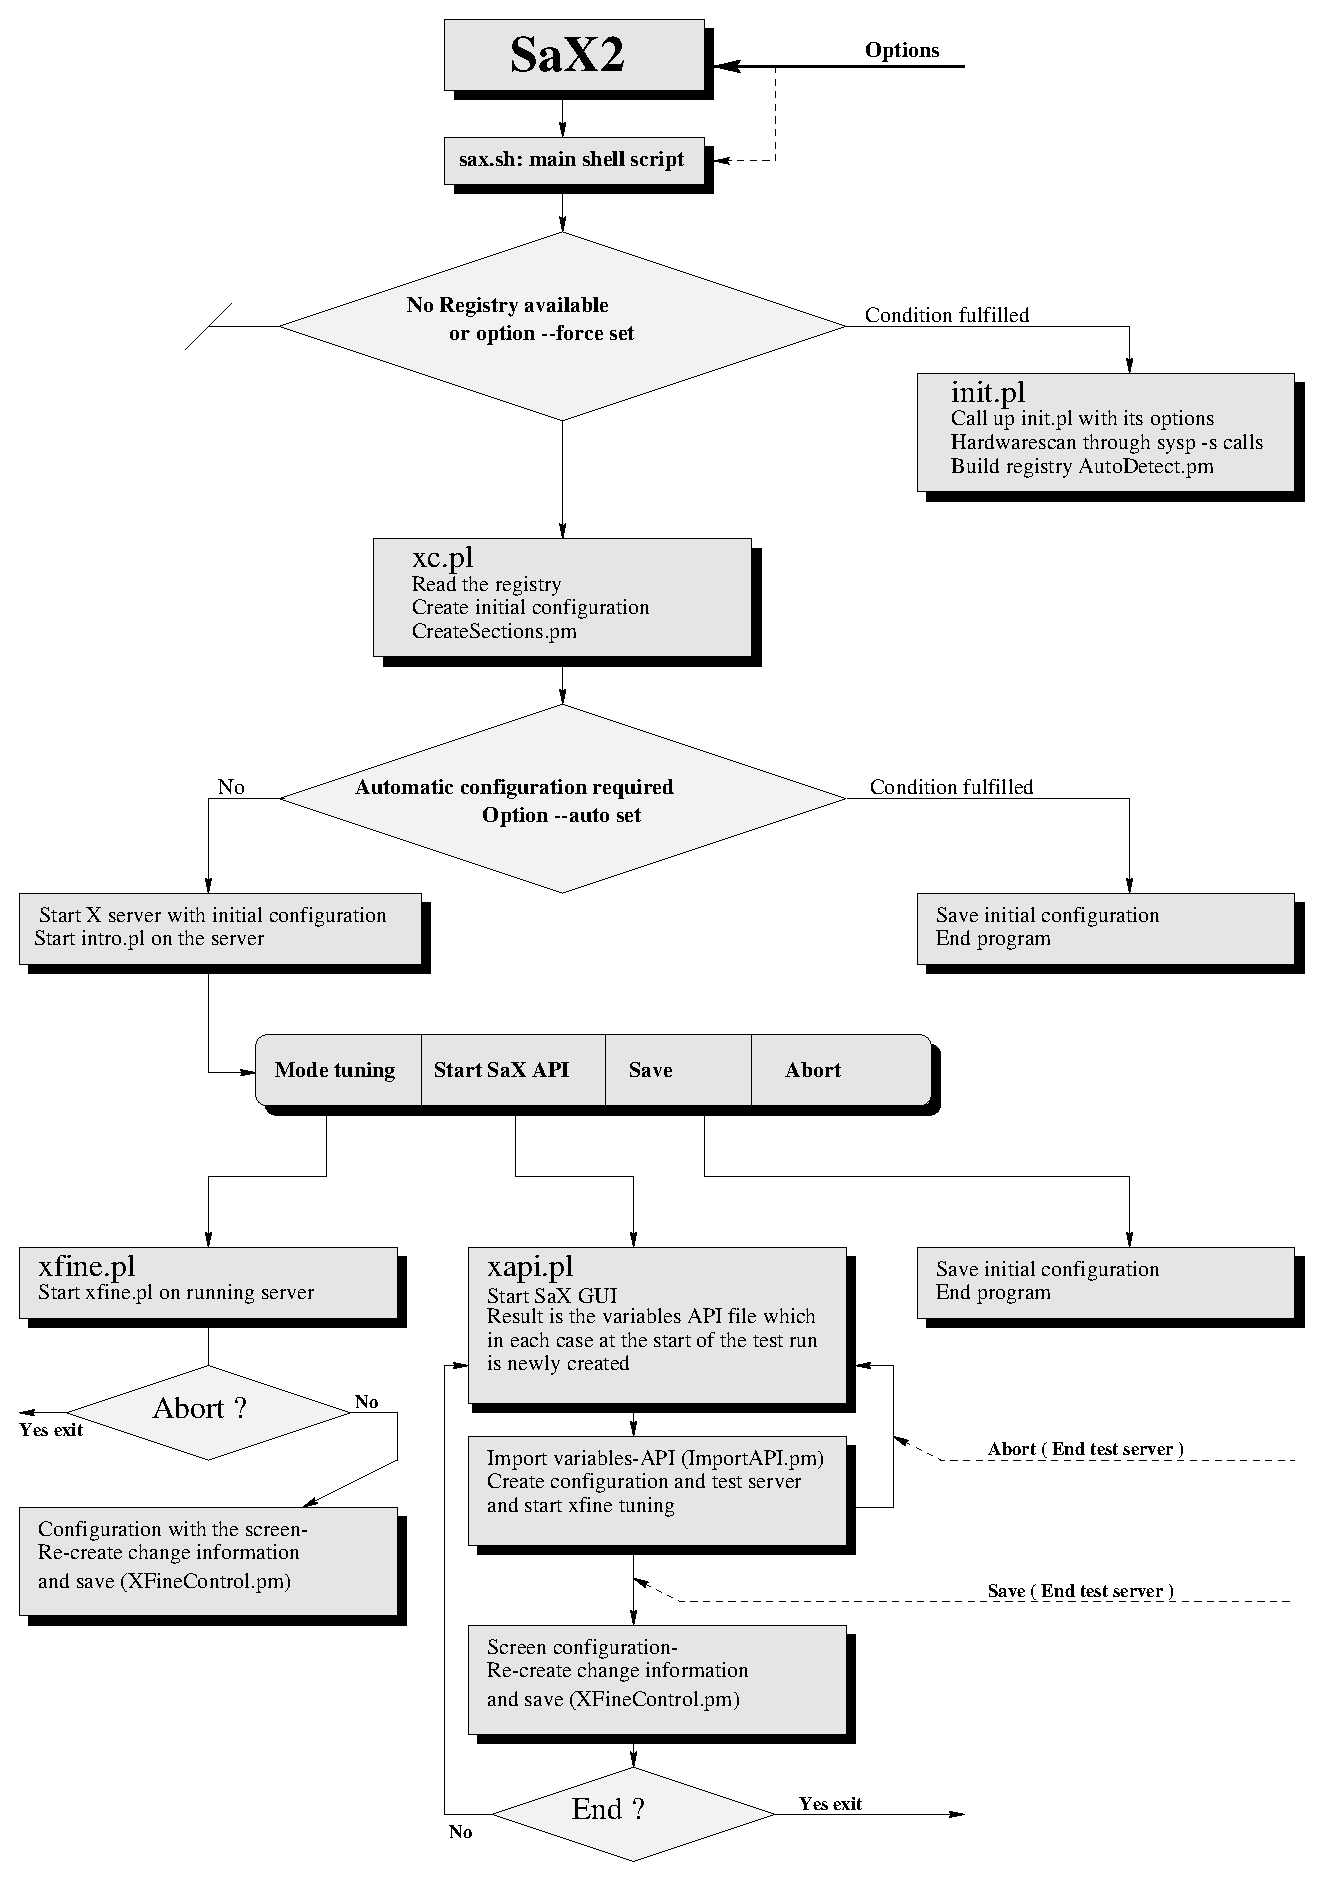
\epsfig{file=pictures/cheme.ps,width=11.5cm}
\caption{SaX2 Flow diagram}
\end{figure}





%%% Local Variables: 
%%% mode: latex
%%% TeX-master: t
%%% End: 

